% https://tex.stackexchange.com/a/17355
% CC BY-SA 3.0 (c) 2011 Matthew Leingang
\documentclass[border=0.8ex,svgnames,tikz]{standalone}
\usepackage{amsmath,mathtools}
\usepackage{fontspec}
\setmainfont{Source Serif 4}
\setsansfont{Source Sans 3}
\setmonofont{Source Code Pro}
\usetikzlibrary{shapes.multipart}
\begin{document}
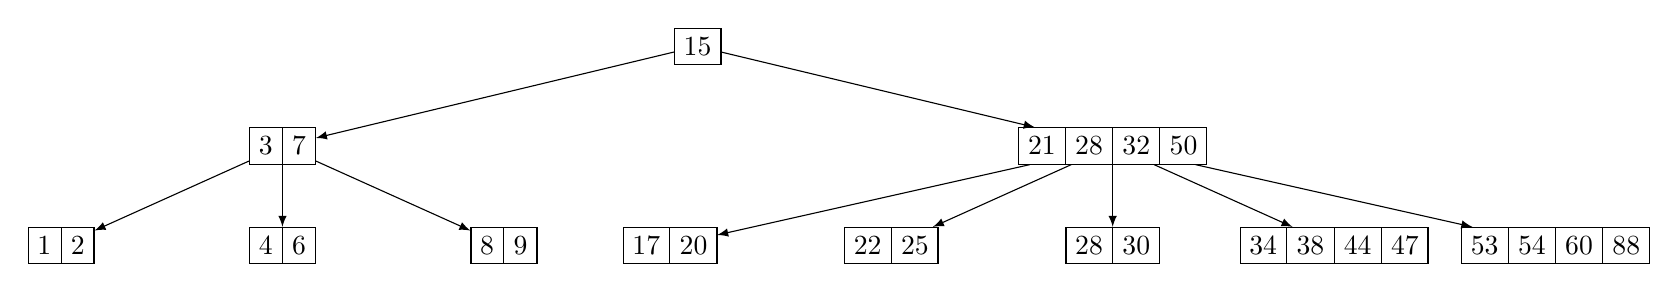
\begin{tikzpicture}[
  level distance=3.6em,
  every node/.style={
    draw,
    rectangle split,
    rectangle split horizontal,
    rectangle split ignore empty parts,
  },
  level 1/.style={sibling distance=15em},
  level 2/.style={sibling distance=08em},
  every path/.style={draw,>=latex},
  ]
  \node{\nodepart{one}15}
  [->]
  child{
    node{\nodepart{one}3 \nodepart{two}7}
    child{ node{\nodepart{one}1 \nodepart{two}2} }
    child{ node{\nodepart{one}4 \nodepart{two}6} }
    child{ node{\nodepart{one}8 \nodepart{two}9} }
  }
  child[missing]
  child{
    node{\nodepart{one}21 \nodepart{two}28 \nodepart{three}32 \nodepart{four}50}
    child{ node{\nodepart{one}17 \nodepart{two}20} }
    child{ node{\nodepart{one}22 \nodepart{two}25} }
    child{ node{\nodepart{one}28 \nodepart{two}30} }
    child{ node{\nodepart{one}34 \nodepart{two}38 \nodepart{three}44
        \nodepart{four}47}}
    child{ node{\nodepart{one}53 \nodepart{two}54 \nodepart{three}60
        \nodepart{four}88}}
  };
\end{tikzpicture}
\end{document}
